\documentclass[journal,12pt,twocolumn]{IEEEtran}
%
\usepackage{setspace}
\usepackage{gensymb}
\usepackage{xcolor}
\usepackage{caption}
%\usepackage{subcaption}
%\doublespacing
\singlespacing
\usepackage{multicol}
%\usepackage{eenrc}
\usepackage{iithtlc}
%\usepackage{graphicx}
%\usepackage{amssymb}
%\usepackage{relsize}
\usepackage[cmex10]{amsmath}
\usepackage{mathtools}
%\usepackage{amsthm}
%\interdisplaylinepenalty=2500
%\savesymbol{iint}
%\usepackage{txfonts}
%\restoresymbol{TXF}{iint}
%\usepackage{wasysym}
\usepackage{amsthm}
\usepackage{mathrsfs}
\usepackage{txfonts}
\usepackage{stfloats}
\usepackage{cite}
\usepackage{cases}
\usepackage{subfig}
%\usepackage{xtab}
\usepackage{longtable}
\usepackage{multirow}
%\usepackage{algorithm}
%\usepackage{algpseudocode}
\usepackage{enumitem}
\usepackage{mathtools}
%\usepackage{stmaryrd}
\usepackage{graphicx}
\usepackage{listings}
\usepackage{circuitikz}
    \usepackage[latin1]{inputenc}                                 %%
    \usepackage{color}                                            %%
    \usepackage{array}                                            %%
    \usepackage{longtable}                                        %%
    \usepackage{calc}                                             %%
    \usepackage{multirow}                                         %%
    \usepackage{hhline}                                           %%
    \usepackage{ifthen}                                           %%
  %optionally (for landscape tables embedded in another document): %%
    \usepackage{lscape}     
\usepackage{url}
\def\UrlBreaks{\do\/\do-}

%\usepackage{wasysym}
%\newcounter{MYtempeqncnt}
\DeclareMathOperator*{\Res}{Res}
%\renewcommand{\baselinestretch}{2}
\renewcommand\thesection{\arabic{section}}
\renewcommand\thesubsection{\thesection.\arabic{subsection}}
\renewcommand\thesubsubsection{\thesubsection.\arabic{subsubsection}}

\renewcommand\thesectiondis{\arabic{section}}
\renewcommand\thesubsectiondis{\thesectiondis.\arabic{subsection}}
\renewcommand\thesubsubsectiondis{\thesubsectiondis.\arabic{subsubsection}}

% correct bad hyphenation here
\hyphenation{op-tical net-works semi-conduc-tor}

\def\inputGnumericTable{}  

\lstset{
language=python,
frame=single, 
breaklines=true
}

\begin{document}
%

\theoremstyle{definition}

\newtheorem{theorem}{Theorem}[section]
\newtheorem{problem}{Problem}
\newtheorem{proposition}{Proposition}[section]
\newtheorem{lemma}{Lemma}[section]
\newtheorem{corollary}[theorem]{Corollary}
\newtheorem{example}{Example}[section]
\newtheorem{definition}{Definition}[section]
%\newtheorem{algorithm}{Algorithm}[section]
%\newtheorem{cor}{Corollary}
\newcommand{\BEQA}{\begin{eqnarray}}
\newcommand{\EEQA}{\end{eqnarray}}
\newcommand{\define}{\stackrel{\triangle}{=}}

\bibliographystyle{IEEEtran}
%\bibliographystyle{ieeetr}



\providecommand{\pr}[1]{\ensuremath{\Pr\left(#1\right)}}
\providecommand{\qfunc}[1]{\ensuremath{Q\left(#1\right)}}
\providecommand{\sbrak}[1]{\ensuremath{{}\left[#1\right]}}
\providecommand{\lsbrak}[1]{\ensuremath{{}\left[#1\right.}}
\providecommand{\rsbrak}[1]{\ensuremath{{}\left.#1\right]}}
\providecommand{\brak}[1]{\ensuremath{\left(#1\right)}}
\providecommand{\lbrak}[1]{\ensuremath{\left(#1\right.}}
\providecommand{\rbrak}[1]{\ensuremath{\left.#1\right)}}
\providecommand{\cbrak}[1]{\ensuremath{\left\{#1\right\}}}
\providecommand{\lcbrak}[1]{\ensuremath{\left\{#1\right.}}
\providecommand{\rcbrak}[1]{\ensuremath{\left.#1\right\}}}
\theoremstyle{remark}
\newtheorem{rem}{Remark}
\newcommand{\sgn}{\mathop{\mathrm{sgn}}}
\providecommand{\abs}[1]{\left\vert#1\right\vert}
\providecommand{\res}[1]{\Res\displaylimits_{#1}} 
\providecommand{\norm}[1]{\lVert#1\rVert}
\providecommand{\mtx}[1]{\mathbf{#1}}
\providecommand{\mean}[1]{E\left[ #1 \right]}
\providecommand{\fourier}{\overset{\mathcal{F}}{ \rightleftharpoons}}
%\providecommand{\hilbert}{\overset{\mathcal{H}}{ \rightleftharpoons}}
\providecommand{\system}{\overset{\mathcal{H}}{ \longleftrightarrow}}
\providecommand{\gauss}[2]{\mathcal{N}\ensuremath{\left(#1,#2\right)}}
	%\newcommand{\solution}[2]{\textbf{Solution:}{#1}}
\newcommand{\solution}{\noindent \textbf{Solution: }}
\providecommand{\dec}[2]{\ensuremath{\overset{#1}{\underset{#2}{\gtrless}}}}
%\numberwithin{equation}{section}
%\numberwithin{problem}{section}

\def\putbox#1#2#3{\makebox[0in][l]{\makebox[#1][l]{}\raisebox{\baselineskip}[0in][0in]{\raisebox{#2}[0in][0in]{#3}}}}
     \def\rightbox#1{\makebox[0in][r]{#1}}
     \def\centbox#1{\makebox[0in]{#1}}
     \def\topbox#1{\raisebox{-\baselineskip}[0in][0in]{#1}}
     \def\midbox#1{\raisebox{-0.5\baselineskip}[0in][0in]{#1}}


% paper title
% can use linebreaks \\ within to get better formatting as desired

%\title{FM Signal Transmission Using Pi}
 
 
%\title{Electrical Circuit Design using Latex}

\title{
\logo{
C Programming through Wiring Pi 
}
} 
 
%
%
% author names and IEEE memberships
% note positions of commas and nonbreaking spaces ( ~ ) LaTeX will not break
% a structure at a ~ so this keeps an author's name from being broken across
% two lines.
% use \thanks{} to gain access to the first footnote area
% a separate \thanks must be used for each paragraph as LaTeX2e's \thanks
% was not built to handle multiple paragraphs
%

%\author{Y Aditya, A Rathnakar and G V V Sharma$^{*}$% <-this % stops a space
%\author{K Prasanna Kumar  %<-this  stops a space
%\thanks{The author is Project Associate in National Resource Centre - IIT Hyderabad
%502285 India e-mail: kk.prassu924@gmail.com 
%}}

\author{K Prasanna Kumar and G V V Sharma %<-this  stops a space
\thanks{The authors are with the Department
of Electrical Engineering, IIT, Hyderabad
502285 India $1^{st}$ e-mail: kk.prassu924@gmail.com, $2^{st}$e-mail: \{gadepall\}@iith.ac.in. 
}}


% make the title area
\maketitle


\tableofcontents

\bigskip

\begin{abstract}
This manual shows how to install Wiring Pi library in Raspberry Pi and control GPIO pins using C program. It helps us to analyze how C programing is used to interact with hardware.  
\end{abstract}
\section{Installation of Wiring Pi}
In this section the installation of wiring pi library in R Pi from github in is explained.\\
\subsection*{Method - 1}
If you do not GIT installed use the following command.
\begin{lstlisting}[frame = single]
 sudo apt-get install git-core
\end{lstlisting}
Download or clone wiring pi from GIT
\begin{lstlisting}[frame = single]
sudo apt-get update
sudo apt-get upgrade
cd 
git clone git://git.drogon.net/wiringPi
or 
git clone https://github.com/PrasannaIITH/WiringPi-1
\end{lstlisting}
Web link (i.e. url) to download wiringpi from GIT
\url{https://github.com/WiringPi/WiringPi}\\

Steps to install wiringpi if it is cloned
\begin{lstlisting}[frame = single]
cd ~/wiringPi
./build
\end{lstlisting}

Steps to install wiringpi if it is downloaded from web link. Downloaded file will be in zip formate, extract it in the home directory.
\begin{lstlisting}[frame = single]
cd file_name
./build
\end{lstlisting}

Type the following manual command to known how to use the gipo utility 
\begin{lstlisting}[frame= single]
man gpio
\end{lstlisting}


Run the gpio command to check the installation
\begin{lstlisting}[frame = single]
gpio -v
gpio readall
\end{lstlisting}

\subsection*{Method - 2}
\begin{lstlisting}
sudo apt-get update
sudo apt-get install gdebi
mkdir WiringPi
cd WiringPi
wget https://github.com/PrasannaIITH/wiringPi/blob/master/wiringpi-2.50-1.deb
sudo gdebi install wiringpi-2.50-1.deb
\end{lstlisting}

\section{Basic programming using Wiring Pi}
Before execution of any programing initialize BCM-GPIO pin numbering by using following command
\begin{lstlisting}[frame = single]
gpio -g mode 17 output
\end{lstlisting}
in the above command '-g' indicates the BCM (Broadcom) pin numbering, 'mode' indicates the mode of operation of pin i.e. \textit{Input/output}. If the BCM pin numbers are not assigned then Pi will take default pin numbering.


\subsection{Control LED blink}
Here is an example experiment of LED blink using broadcom pin number 17.
\begin{figure}[h!]
\centering
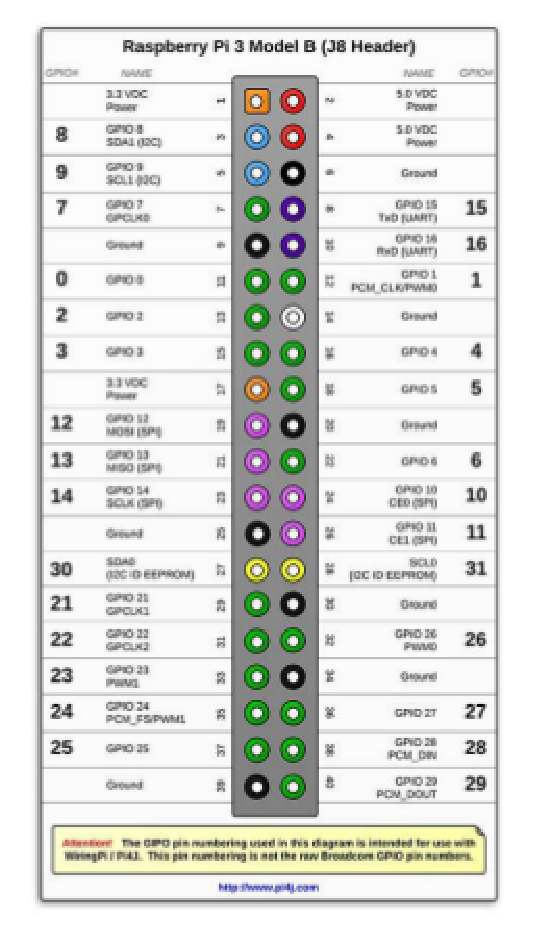
\includegraphics[scale=0.6]{figs/Pindiagram}
\caption{Schematic diagram of RPi 3B pin diagram \cite{b2}}
\end{figure}

\begin{lstlisting}[frame = single]
#include <stdio.h>
#include <wiringPi.h>

#define	LED	0
// The above command tell that 
// LED Pin - wiringPi pin 0 is BCM_GPIO pin 17.

int main (void)
{
  printf ("Raspberry Pi blink\n") ;

  wiringPiSetup () ;
  // setup function due Broadcom numbering.
  pinMode (LED, OUTPUT) ;

  for (;;)
  {
    digitalWrite (LED, HIGH) ;	// On
    delay (500) ;		// mS
    digitalWrite (LED, LOW) ;	// Off
    delay (500) ;
  }
  return 0 ;
}
\end{lstlisting}
The above program should be saved as .c file. Now compile \& run the program 
\begin{lstlisting}[frame= single]
gcc filename.c -o filename.out -l wiringPi
sudo ./output_filename
\end{lstlisting}

\begin{figure}[h!]
\centering
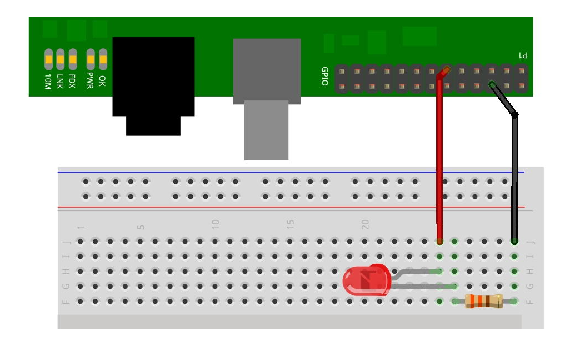
\includegraphics[scale=0.9]{figs/blink}
\caption{Schematic of LED connected to Pi}\cite{b1}
\end{figure}

\subsection{Display of Numbers on SSD}
Here LEDs are controlled using push button. Connect the circuit as per the schematic diagram.
\begin{figure}[h!]
\centering
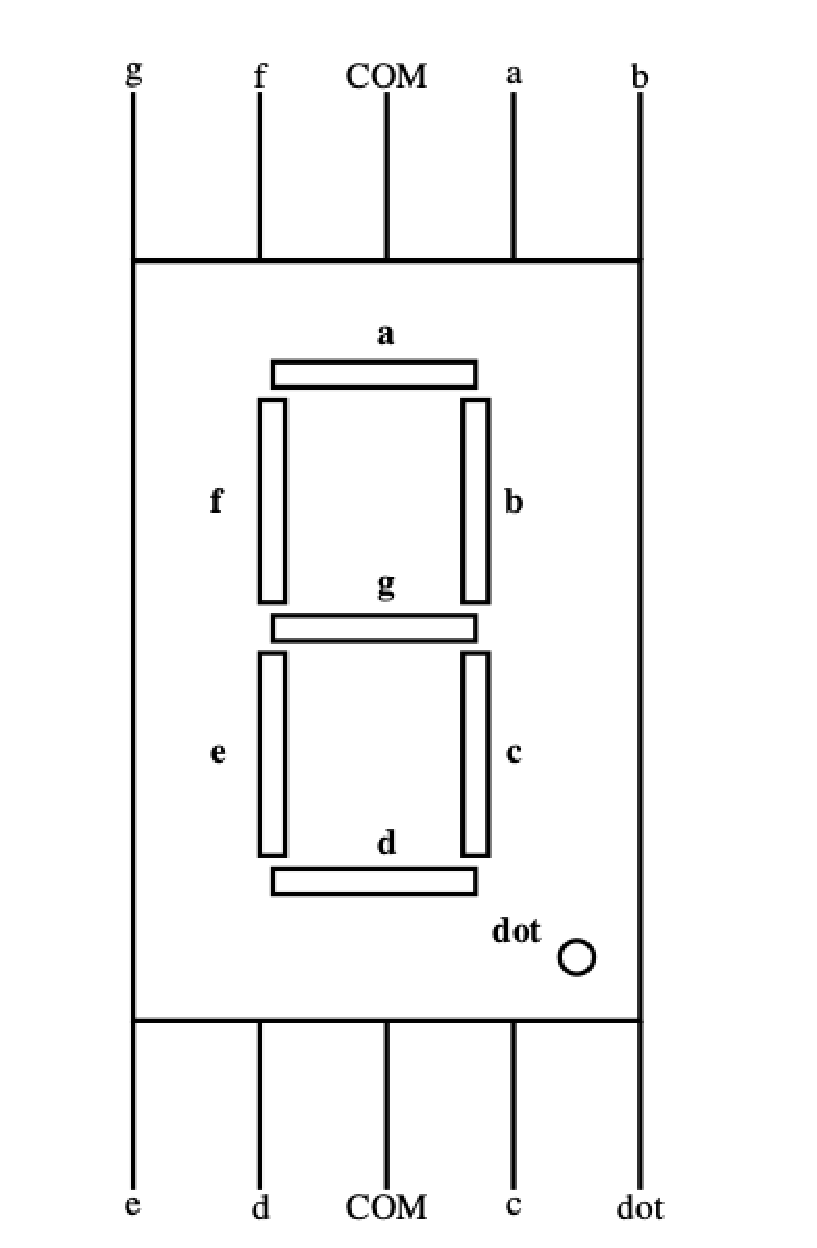
\includegraphics[scale=0.5]{figs/ssd.eps}
\caption{Schematic diagram of Seven Segment Display \cite{b2}}
\end{figure}

\begin{lstlisting}[frame=single]
#include <stdio.h>
#include <wiringPi.h>

int main(void)
{
int a = 1
int b = 1
int c = 1
int d = 1
int e = 1
int f = 1
int g = 0

wiringPisetup();
    pinMode(2, OUTPUT);  
    pinMode(3, OUTPUT);
    pinMode(4, OUTPUT);
    pinMode(5, OUTPUT);
    pinMode(6, OUTPUT);
    pinMode(7, OUTPUT);
    pinMode(8, OUTPUT);

for (;;)
{

  digitalWrite(2, a); 
  digitalWrite(3, b); 
  digitalWrite(4, c); 
  digitalWrite(5, d); 
  digitalWrite(6, e); 
  digitalWrite(7, f);     
  digitalWrite(8, g); 

}

return 0;
}


\end{lstlisting}  
Save the program file as .c file. Run \& compile the the program as above.

\section{Conclusion}
By this we can understand that how a basic C programing will help us to talk with the real world hardware. WiringPi is released under the GNU Lesser Public License version 3. For more information visit \url{http://www.wiringpi.com/}.

%\begin{lstlisting}
%import RPi.GPIO as GPIO
%from time import sleep
%GPIO.setmode (GPIO.BOARD)
%GPIO.setup (11,GPIO.OUT)
%GPIO.setup (7,GPIO.OUT)
%
%while 1:
%try:
%GPIO.output(11,GPIO.HIGH)
%sleep (1)
%GPIO.output (11,GPIO.LOW)
%sleep (1)
%GPIO.output(7,GPIO.HIGH)
%sleep (1)
%GPIO.output (7,GPIO.LOW)
%sleep (1)
%except KeyboardInterrupt:
%GPIO.cleanup()
%\end{lstlisting}

\begin{thebibliography}{00}
\bibitem{b1}Wiring Pi- GPIO Interface library for the Raspberry Pi, url{http://www.wiringpi.com/}. 
\bibitem{b2} Sunfounder, Raspberry pi tutorial - 'Lesson 2 Controlling an LED by a Button' \url{https://www.sunfounder.com/}. Demo video link \url{https://www.youtube.com/watch?time_continue=4&v=y3Pv7--6eik}.
\end{thebibliography}
\end{document}
